\documentclass{ctexart}
\usepackage{amsmath}
\usepackage{amssymb}
\usepackage[a4paper, total={6in, 8in}]{geometry}
\usepackage{float}
\usepackage{subfigure}
\usepackage{graphicx}

\title{FEM - 第三周作业1 二次有限元}
\author{SA23001071 杨哲睿}
\ctexset{
  section/format    += \sffamily\raggedright,
}

\begin{document}
\maketitle

\section{Introduction}
编写程序求解两点边值问题:
\begin{equation}
  \begin{cases}
    - u'' = f & 0 < x < 1\\
    u(0) = u(1) = 0
  \end{cases}
\end{equation}
选取等距网格剖分,有限元空间选取分段二次多项式空间 $V_h$,选取准确解 $u(x) = (x-1) \sin (x)$ 算出满足方程的$f(x)$。

\section{Method}


定义双线性型$a(u, v) = \int_0^1 u' v' \mathrm dx$,内积$(f, g) = \int_0 ^ 1 f \cdot g \mathrm dx$。那么变分问题是

\textit{找 $u\in V = \{ v\in H^1[0, 1], v(0) = v(1) = 0\}$,使得$a(u, v) = (f, v), ~ \forall v \in V$都成立.}

实验中采用等距网格划分,单元数为 $N$,节点处的值为$u_i = u(x_i) = u(i h)$,$h = 1/N$。选取分段二次多项式空间。标准单元形函数为:
\begin{eqnarray}
  \phi_0 = \begin{cases}
    (2 x - 1) (x-1) & 0 \le x \le 1\\
    0&\text{otherwise}
  \end{cases}\\
  \phi_1 = \begin{cases}
    4 x (1-x) & 0 \le x \le 1\\
    0&\text{otherwise}
  \end{cases}\\
  \phi_2 = \begin{cases}
    (2 x - 1) x & 0 \le x \le 1\\
    0&\text{otherwise}
  \end{cases}\\
\end{eqnarray}
局部基函数:
\begin{eqnarray}
  \phi_0^i = \phi_0(\frac{x-x_{i-1}}{x_i-x_{i-1}})\\
  \phi_1^i = \phi_1(\frac{x-x_{i-1}}{x_i-x_{i-1}})\\
  \phi_2^i = \phi_2(\frac{x-x_{i-1}}{x_i-x_{i-1}})\\
\end{eqnarray}

全局基函数共$2n+1$个,为:
\begin{eqnarray}
  \phi_i = \phi_2^i + \phi_0^{i+1} = \begin{cases}
    \left(2\frac{x-x_{i-1}}{x_i - x_{i-1}} -1\right)\left(\frac{x-x_{i-1}}{x_i - x_{i-1}}-1\right) & x_{i-1} \le x \le x_i\\
    \left(2\frac{x_{i+1}-x}{x_{i+1} - x_{i}} -1\right)\left(\frac{x_{i+1}-x}{x_{i+1} - x_{i}}\right) & x_{i} \le x \le x_{i+1}\\ 
    0 & \text{otherwise}
  \end{cases}\quad \forall i = 1, 2, ..., N-1\\
  \phi_{i+1/2} = \begin{cases}
    \phi_1^{i} = 4 \frac{x - x_{i-1}}{x_i - x_{i-1}}\left(1-\frac{x - x_{i-1}}{x_i - x_{i-1}}\right)  & x_{i} \le x \le x_{i+1}\\
    0 & \text{otherwise}
  \end{cases}\quad \forall i = 0, 1, ..., N-1
\end{eqnarray}
形状如下图所示
\begin{figure}[H]
    \centering
    \subfigure[$\phi_i$]{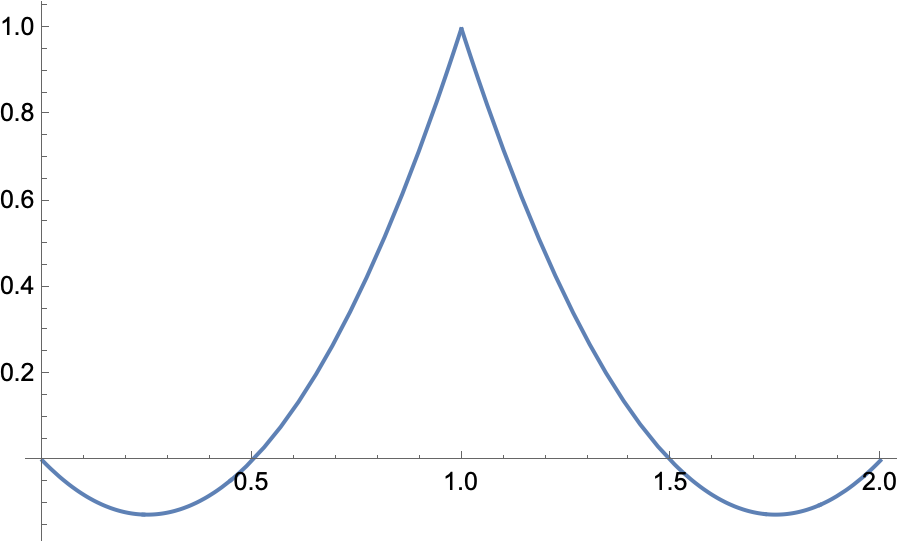
\includegraphics[width=0.45\linewidth]{./global1.png}}
    \subfigure[$\phi_{i+1/2}$]{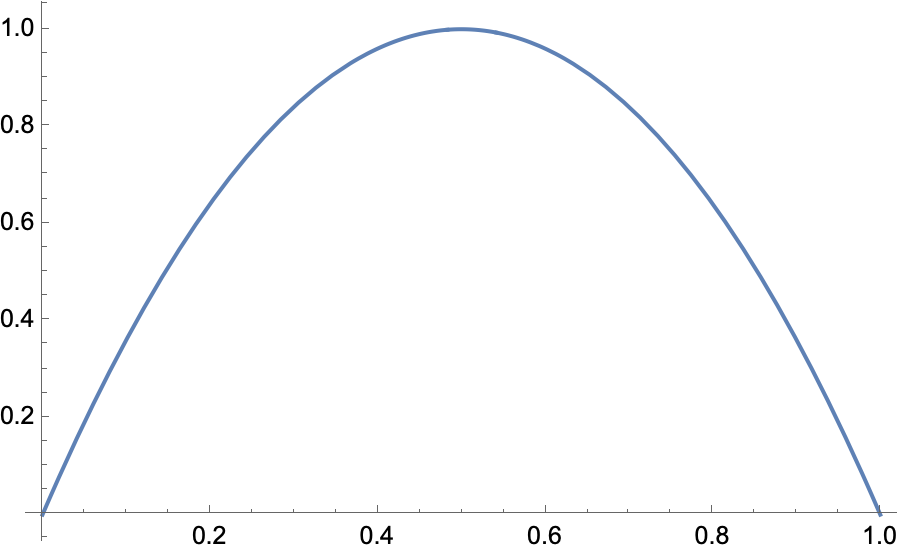
\includegraphics[width=0.45\linewidth]{./global2.png}}
\end{figure}

局部刚度矩阵的系数计算:
\begin{equation}
    K_{l, m} =
     \int_{x_{i-1}} ^ {x_{i}} {\phi^{i}_l}' {\phi^{i}_m}' \mathrm dx 
     = \frac{1}{h}\int_0^1 \phi_l ' \phi_m ' \mathrm dx
\end{equation}
因此局部刚度矩阵为:
\begin{equation}
    K = \frac{1}{h} \begin{pmatrix}
        \frac{7}{3} & -\frac{8}{3} & \frac{1}{3}\\
        -\frac{8}{3} & \frac{16}{3} & -\frac{8}{3}\\
        \frac{1}{3} & -\frac{8}{3} & \frac{7}{3}
    \end{pmatrix}
\end{equation}

全局刚度矩阵:
\begin{equation}
    A = \frac{1}{h}\begin{pmatrix}
          \frac{16}{3} & -\frac{8}{3} & 0 & \cdots   & 0 & 0 \\
         -\frac{8}{3}  & \frac{14}{3} & -\frac{8}{3} & \frac{1}{3} & \cdots &0 & 0\\
         0             & -\frac{8}{3} & \frac{16}{3} & \frac{8}{3} & \cdots & 0 & 0\\
         0             & \frac{1}{3}  & -\frac{8}{3} & \frac{14}{3} & \cdots & 0 & 0\\
          0 & 0 & 0 & \vdots & \ddots & \vdots &0 \\
          0 & 0 & 0 & 0&  \cdots& \frac{14}{3} & -\frac{8}{3}\\
          0 & 0 & 0 & 0& \cdots& -\frac{8}{3} & \frac{16}{3}\\
    \end{pmatrix}\in \mathbb{R}^{(2N -1) \times (2N-1)}
\end{equation}

计算 $(f, \phi_j)$ 得:
\begin{equation}
\begin{aligned}
    f_j &\approx \frac{1}{3} h f(x_j)\\
    f_{j+1/2} & \approx \frac{2}{3} h(x_{j+1/2})
\end{aligned}
\end{equation}

因此为求解节点上的值,只需要求解出 $A U = F$,其中:
\begin{equation}
    U  = \begin{pmatrix}
        u_{1/2}\\
        u_1\\
        \vdots\\
        u_{N-1}\\
        u_{N-1/2}
    \end{pmatrix},
    \quad
    F = \begin{pmatrix}
        f_{1/2}\\
        f_1\\
        \vdots\\
        f_N\\
        f_{N-1/2}
    \end{pmatrix}
\end{equation}


\section{Results}

对于求得的系数,先进行插值,然后进行梯形公式数值积分。可以看出,有限元方法的$L^2$误差是三阶的,$H^1$误差是二阶的。
\begin{table}[H]
  \caption{\label{table.label} 误差分析} \centering
  \bigskip
  \begin{small}
  \begin{tabular}{|c|cc|cc|}
    \hline
    % after \\: \hline or \cline{col1-col2} \cline{col3-col4} ...
    n &$L^2 $ error & order &$ H^1$ error & order\\\hline
    10 & 8.0262e-6 & ---  & 1.6270e-03 & --- \\
    20 & 1.0015e-6 & 3.00 & 4.1150e-04 & 1.98\\
    40 & 1.2514e-7 & 3.00 & 1.0293e-04 & 1.99 \\
    80 & 1.5640e-8 & 3.00 & 2.5476e-05 & 2.00\\\hline
  \end{tabular}
  \end{small}
\end{table}

\section{Discussion}

利用误差方程可知:
\begin{equation}
  (u - u_h, v) = 0\quad \forall v \in V_h
\end{equation}
因也就是说:
\begin{equation}
  \| u_h - u \| \le \| v - u \| \quad\forall v \in V_h
\end{equation}
不妨考虑 $u_I$ 为$u$的分片二次插值函数。在区间$[a,b]$上,满足:
\begin{equation}
  u(a) = u_I(a)\quad u(b) = u_I(b) \quad u(\frac{a+b}{2}) = u_I(\frac{a+b}{2})
\end{equation}
对于 $f = u-u_I$,在$[a,b]$有三个零点,从而$f''$在$[a,b]$有一个零点。令 $M = \max_{x \in [a,b]} |f'''(x)| = \max_{x\in[a,b]} |u'''(x)|$
\begin{eqnarray}
  \sup | f'' | < C (b-a) M\\
  \sup | f' |  < C (b-a)^2 M\\
  \sup | f |   < C (b-a)^3 M
\end{eqnarray}
即对于每个区间$[x_{i-1}, x_{i}]$,有:
\begin{eqnarray}
  \int_{x_{i-1}}^{x_i} |f|^2 \mathrm dx < C h^7 M\\
  \int_{x_{i-1}}^{x_i} (|f|')^2 \mathrm dx < C h^5 M
\end{eqnarray}
对所有区间求和可知:
\begin{eqnarray}
  \int_{0}^{1} |f|^2 \mathrm dx < C h^6 M\\
  \int_{0}^{1} |f|^2 \mathrm dx < C h^4 M\\
\end{eqnarray}
那么:
\begin{eqnarray}
  \| u_h - u \|_{L^2} < \| u_I - u \| = O(h^3)\\
  \| u_h' - u' \| \le \| u_I' - u' \| = O(h^2)\\
\end{eqnarray}
即该有限元方法对$L^2$误差有3阶精度,对$H^2$误差有2阶精度。

\end{document}
